\section{YuE2 legacy spectral replication and separator correction}

This separate replication uses the historical first-30-second, 44.1\,kHz
stereo representation, including padding for two short YuE2 originals. It is
not interchangeable with the native-center30 cohort. Five hundred human and
500 YuE2 recordings contribute full-mix descriptors and raw/corrected vocal
descriptors; the separator calibration is reused from external MUSDB oracle
vocals, not estimated from this AI/human comparison.

\subsection{Fixed within-generator comparison}
The fixed development/test split has 400/100 recordings per class. Human
artist groups and YuE2 source-song groups are disjoint across the split, but
the human test recordings have been used in historical experiments. Moreover,
YuE2 appears in development. Thus this is a within-generator historical-holdout
comparison, not a new external or held-generator validation.

The original legacy ridge implementation fits targets $2y-1$ with penalty
$\alpha=10$ and threshold zero, using training-only means and scales. An
initial adapter incorrectly assumed the later Native30 threshold of 0.5;
an independent balanced-accuracy calculation stopped that run. The preserved
v2 adapter restores the original zero threshold; it does not optimize a
threshold using test outcomes. The original row-wise development cross-validation
is not presented here as group-independent evidence.

\begin{table}[htbp]
\centering
\caption{The fixed 22-statistic spectral representations on 100 human and
100 YuE2 test recordings. All 18 pre-existing full-mix/vocal and frequency-band
representations are retained in the companion CSV; these three rows are a
matched representation comparison, not the top-ranked outcomes.}
\begin{tabular}{lrrrr}
\toprule
Representation & BA & AUC & Specificity & Sensitivity \\
\midrule
Full mix & 0.925 & 0.9706 & 0.940 & 0.910 \\
Raw vocal & 0.950 & 0.9837 & 0.930 & 0.970 \\
Corrected vocal & 0.950 & 0.9832 & 0.930 & 0.970 \\
\bottomrule
\end{tabular}
\end{table}

In this matched comparison, separator correction does not change balanced
accuracy and changes AUC only slightly. These point estimates do not establish
statistical equivalence, causal attribution, or benefit on unseen generators.
In particular, source composition, production, mastering, vocal activity and
excerpt position can contribute to the observed high discrimination.

\subsection{Average difference spectrogram}
Figure~\ref{fig:yue2difference} compares class-average dB spectra on the locked
subset. The STFT uses 4096 samples and a 1024-sample hop; displayed frequencies
are aggregated into 128 logarithmic bands from 300\,Hz to 20\,kHz. Shape panels
subtract each frame's mean across these bands. Clips are aligned by excerpt
time, not by musical phrase or vocal onset. The marked time dependence therefore
requires caution: the plot does not isolate a stationary generator fingerprint.
Subtracting a shared frequency response from both classes also need not remove
their class contrast; the correction is not a learned AI-minus-human template.

\begin{figure}[p]
\centering
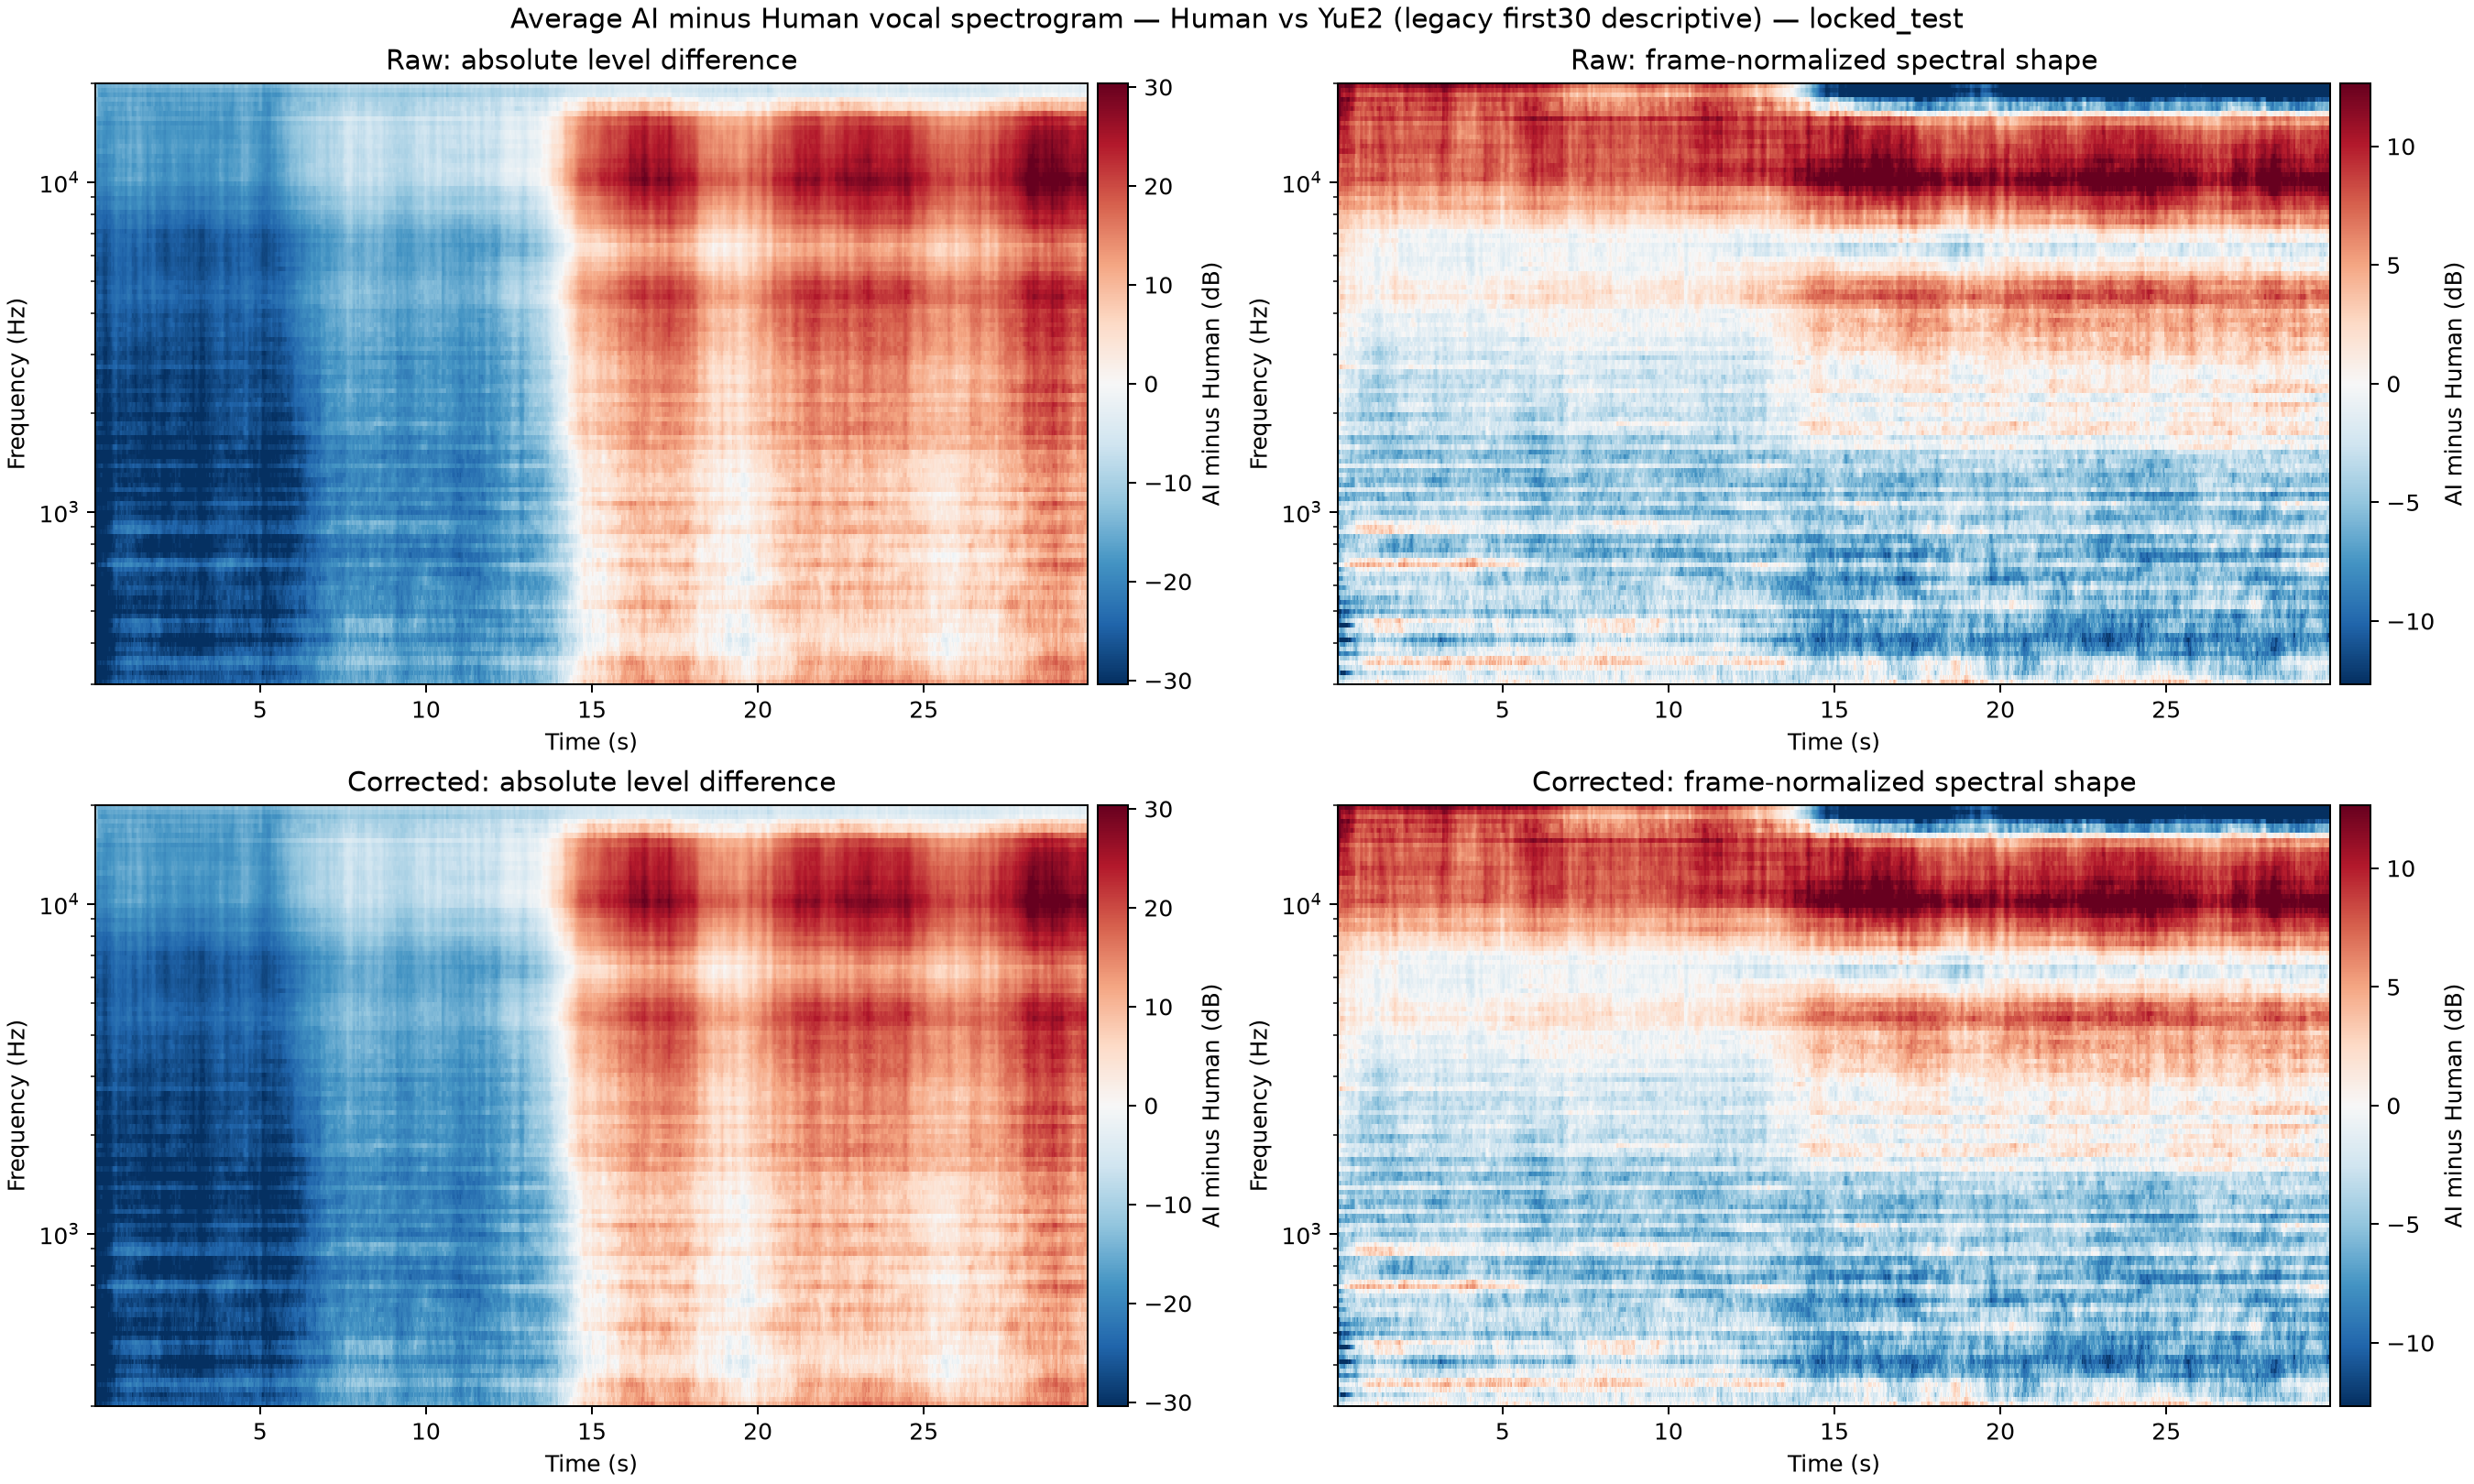
\includegraphics[width=\textwidth]{figures_yue2/average_difference_spectrogram_locked_test.png}
\caption{YuE2 minus human mean vocal spectrograms. Red indicates greater AI
energy or relative band level; blue indicates the reverse. Raw and externally
corrected panels retain broadly similar contrasts. The two classes are not
waveform- or phrase-aligned. This is descriptive visualization, not a classifier
test statistic or evidence of intrinsic AI causation.}
\label{fig:yue2difference}
\end{figure}

\subsection{Retained code and outputs}
Under the report root
\path{/Users/yi/Documents/report/music_ai_detection_20260912/current_results/},
\path{legacy_spectral_measurement_v1/} retains the metrics, frequency vectors,
three cohort heatmaps, numerical maps and input bindings;
\path{legacy_fullmix_v1/} retains the full-mix control;
\path{legacy_spectral_locked_v2/} retains all fitted parameters and predictions;
\path{legacy_spectral_report_v2/all_representations.csv} gives all 18 results.
The failed first adapter is retained in
\path{legacy_spectral_locked_v1_failed/}. Local product hashes were verified
against their producing COMMIT records before this chapter was written.
Relevant source scripts are \path{run_legacy_spectral_measurement_v1.py},
\path{extract_legacy_fullmix_v1.py}, \path{evaluate_legacy_spectral_locked_v2.py},
and \path{report_legacy_spectral_locked_v2.py}, in the YuE2 extension directory.
